\section{Caratterizzazione della strumentazione}%titolo provvisorio
Per ottenere misurazioni ottimali, è stato necessario un lavoro preliminare per l'ottimizzazione della catena elettronica. I parametri regolabili includono: la tensione operativa dei due fotomoltiplicatori, il tempo di shaping per la modellazione dei segnali, la soglia $E_{\text{low}}$ e l'apertura $\Delta E$ della finestra del modulo ORTEC AMP\&SCA.
\subsection{Tensione di lavoro e shaping time}%l'italiano è orribile ma prima scrivo tutto poi cercherò di migliorare la forma, scusate ;(
Dopo aver svolto tutti i collegamenti tra i vari stadi elettronici esposti nella sezione (\ref{Elettronica nucleare}) si è collegato l'oscilloscopio all'uscita amplificata e formata del rivelatore A in modo da visualizzare il segnale uscente dopo l'amplificazione e la formazione. Dall'oscilloscopio è stato possibile eseguire un'ottimizzazione qualitativa direttamente sul segnale aumentando o diminuendo la tensione fornita al fotomoltiplicatore accoppiato con lo scintillatore e variando lo shaping time. In questo modo è stato possibile ricercare un segnale ottimale creando una situazione di compromesso tra la stabilità e la largezza. Il metodo è stato il seguente: stando attenti a non saturare il segnale si è aumentata la differenza di potenziale fornita dal generatore per aumentare l'ampiezza del segnale. Successivamente attraverso due manopole presenti nel modulo ORTEC RESEARCH AMPLIFIER è stato possibile modificare la  pendenza di risalita e discesa in modo tale da stringere il segnale. La tensione impostata per il primo rivelatore è stata scelta a $V_A=329\,\unit{V}$.

Svolgendo lo stesso procedimento per il secondo rivelatore è stata scelta come tensione $V_B=500\,\unit{V}$. Durante quest'ultimo processo si sono riscontrati alcuni problemi in quanto il rumore ambientale rendeva il segnale instabile e inutilizzabile. Per risolvere questo problema è stata aumentata la tensione fornita al fotomoltiplicatore in quanto questa agisce direttamente sul segnale prodotto dallo scintillatore. Tuttavia, a tensioni superiori a quella impostata, il segnale tendeva a saturare, motivo per cui è stata prestata particolare attenzione a evitare questa condizione.
\subsection{Calibrazione}\label{Sez calibrazione}
Il prossimo passo per ottimizzare la catena elettronica è quello di calibrare in energia entrambi i rivelatori. Infatti, il segnale di tensione analogico viene converito, tramite un Analog to Digital Converter (ADC), in un segnale digitale. Successivamente attraverso il Multy-Channel-Analyzer (MCA) i segnali vengono inseriti in un istogramma. Per questo motivo è necessario correlare la posizione nell'istogramma con il valore di energia rilasciata nel rivelatore, ovvero effettuare una calibrazione energetica. 

Questo può essere fatto utilizzando una sorgente avente picchi caratteristici dal valore noto e registrando la loro posizione nello spettro in canali. Le sorgenti utilizzate sono:
\begin{itemize}
    \item $\ch{^{22}Na}$ $(511\,\unit{keV})$;
    \item $\ch{^{137}Cs}$ $(661\,\unit{keV})$;
    \item $\ch{^{22}Ne}$ $(1274\,\unit{keV})$.
\end{itemize}
L'analisi dei picchi è affrontata nella sezione analisi dati (\ref{sez analisi dati calibrazione})
\subsection{Regolazione della finestra di energia}
Un altro passaggio fondamentale prima di iniziare con le misure è impostare la finestra di energia sul rivelatore B. Questo procedimento è fondamentale in quanto durante le misure i due rivelatori sono messi in coincidenza e per studiare l'effetto Compton si utilizzano i fotoni back-to-back prodotti dall'annichilazione del positrone con un elettrone. Di conseguenza attraverso il modulo SCA si può regolare la finestra di apertura in modo che sia centrata attorno al picco da $511\,\unit{keV}$. Questo permette al secondo rivelatore di essere utilizzato come ingresso di gate nel MCA. 

Sperimentalmente, con la sorgente posizionata al centro dell'apparato, è stato collegato il rivelatore B in modo tale da visualizzare lo spettro prodotto all'interno del software MAESTRO. Attraverso due manopole è stato possibile modificare la soglia e l'apertura della finestra. Visualizzando in tempo reale il formarsi dello spettro sullo schermo è stato possibile aggiustare i due parametri in modo tale da visualizzare solo il picco fotoelettrico. Durante questo pocedimento si è stata dedicata particolare attenzione a due fattori principali: la finestra non può essere troppo larga altrimenti si inquina lo spettro acquisito con coincidenze casuali, dall'altra parte non la si può stringere troppo per non abbattere eccessivamente il rate. Dopo aver impostato la finestra è stato necessario verificare che il segnale del fotone rilevato all'interno dello scintillatore A e il segnale logico di gate fossero nello stesso intervallo di tempo. Per fare questo è stato collegato al primo canale dell'oscilloscopio il segnale amplificato e formato del rivelatore A e nel secondo canale il segnale logico di gate come è possibile osservare nella fig. \ref{fig:osc}.
 %IMMAGINE osc
\begin{figure}[htp!]
  \centering
  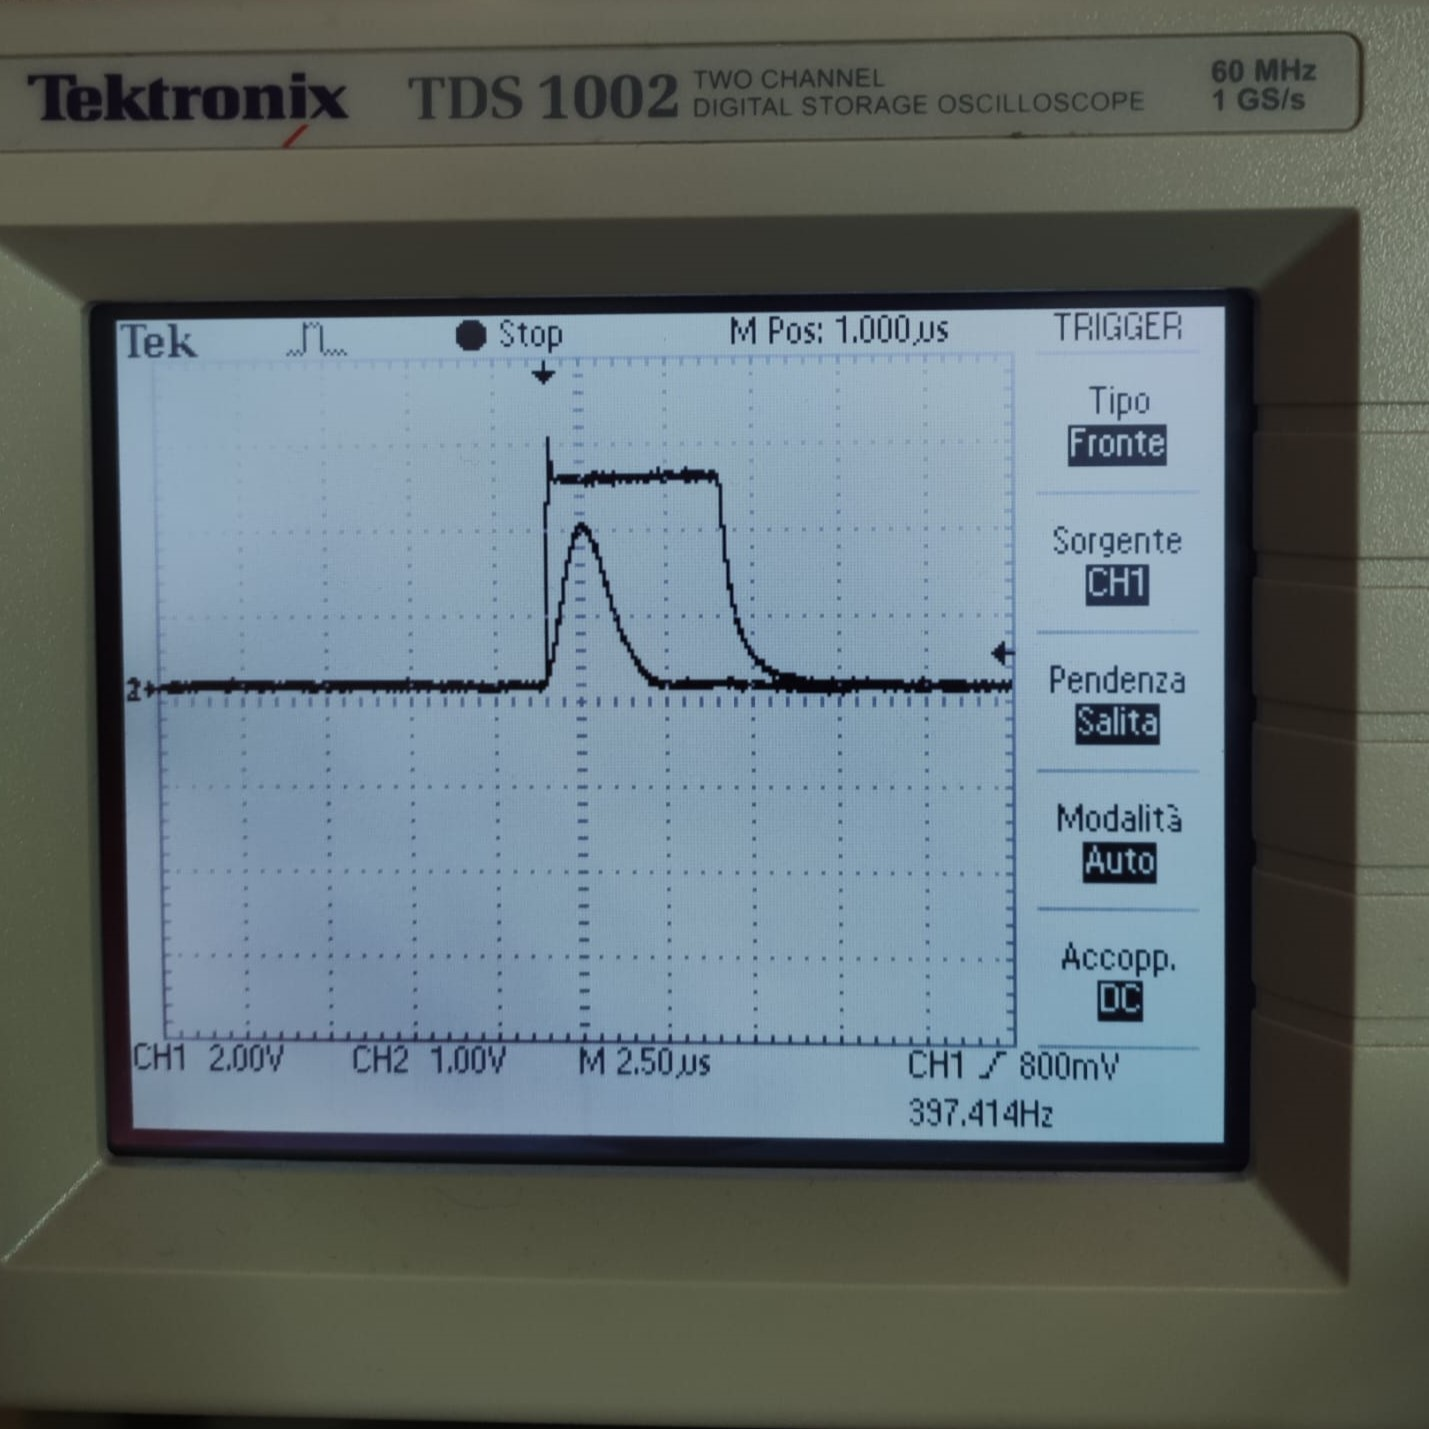
\includegraphics[scale=0.2]{Caratterizzazione della strumentazione/osc.jpg} 
  \caption{In questa immagine è possibile visualizzare la sovrapposizione del segnale del rivelatore A e del segnale logico di gate.}
  \label{fig:osc}
\end{figure}